\section{Week 03}

\subsection{03/08/2015}

\textbf{Other leptons Whizard simulations}

We have copied and Marlin all the other simulations files with one leptons (muons or electrons) in the final state.\\
We would like to analyze the energy-angle distribution to understand if the boundary effect are due to some diagrams which interferes (only in the electrons case) or if they are due to something else.

\textbf{Likelihood fit}

After a lesson about the likelihood and how to fit an histogram by finding the minimum of the likelihood (thanks to Patrick), we started fitting our energy-angle distribution for the electrons with a model $S_0 + a f_1$, where $S_0$ is the standard model distribution and $f_1$ is a BSM correction.\\

We have started from two histograms of $S_0$ and $f_1$ with 200 bins in each dimension and reduced energy between 0.114246 and 1, and $cos\theta$ between -1 and 1 (obviously).\\ We have then normalized the distribution so we can use them as probability density function. So we have reproduced our distribution with these settings and use the likelihood formula:
\[L=-\sum_{events} log(S_0+a f_1) = -\sum_{bins} N_{bin} log(S_0+a f_1)\]
\[L'=-\sum N \frac{f_1}{S_0 + a f_1}  and  L''= \sum N \frac{f_1^2}{(S_0 + a f_1)^2}\]

where N is the number of entries in the selected bin of the montecarlo histogram, and $S_0$ and $f_1$ are the numbers of the entries in the histograms of the probability density function.

Then we could use the tangent method to find iteratively the minimum value (that we expect to be 0).
\[a_0 = a - \frac{L'(a)}{L''(a)}\]

and after all we can estimate the error with \[\sigma = \sqrt{\frac{1}{L''(a_0)}}\]

We have found some errors while calculating the Likelihood and its derivatives cause to the fact that $S_0$ and $f_1$ became very near to 0 in some points. We don't now how to solve yet.

\subsection{04/08/2015}

\textbf{TChain}

We have just discovered a new method to process a lot of Root files containing tree without using glob.
We simply need to define a TChain object:\\
mychain = TChain("MyTreeName")
where MyTreeName is the name of the trees inside the root files.\\
Then we can add all the root files to the chain by using:
mychain.Add("*.root")\\
and then we can loop on all the events dealing mychain as a tree.

\textbf{Likelihood fit part 2}

We found the problem in the code: strangely, if we look to the $S_0$ and $f_1$, we find that the bins (0,*) and (*,0) contains exactly 0 entries. So during the calculation of the derivatives we find several problems in dividing by zero. We solve the problem by simply don't consider these bins. The result is pretty strange because, starting with an initial value of a=0.1 we obtain a result of $a=0.2 \pm 0.01$ with a first derivative very close to zero. This result is only quite reasonable because we expect something close to zero, with 0 into the errorbar.

After a little time we found out that the first bins (*,0) and (0,*) and the last bins (*,201) and (201,*) are the overflow and the underflow of the histograms, so we need to use the method GetBinContent on the bin between 1 and 200 in both directions. The result hasn't changed and we tried to plot the marginal distributions. But this result is not satisfactory.

\subsection{05/08/2015}

\textbf{Physics lesson at Gigi's home}

We have attended a physics lesson at Gigi's home about how to do physics at e+e- colliders.

\subsection{06/08/2015}

\textbf{Leptons tree and effective invariant mass}

We have created 6 trees (one for each possible lepton in the final state) with only the variables we need. In particular there are the energy (and reduced energy), the three component of the momentum, the polar angle, and the invariant mass of the two electrons after radiating photons. This invariant mass is the effective energy at which the collisions happen, and the mean is 363.7 GeV. 

\subsection{07/08/2015}

\textbf{Corrections to the likelihood}

Together with Patrick, we realized that the likelihood we defined on Monday 03/08/2015 was not correct. In fact, the normalization factor that turns the cross sections into the probabilities depends on the parameter $a$, and we have also to consider the probability that our MonteCarlo generator produced $N$ events, if the mean value of events is $\mu$.
Let $S_{tot}$, $f_{tot}$ and $N_{tot}$ be the sum of the contents of the bins in our range of study (we may want to make some cuts in the values of $\cos\theta$ and the reduced energy $x$) for the Standard Model cross section, the correction-to-SM cross sections, and the number of events generated by Whizard. Let the luminosity (integrated over the experiment time) be $K$. Then, the probability of having $N$ events produced in our range of study is:
\[
\frac{\mu^Ne^{-\mu}}{N!} \quad\rightarrow\quad \frac{e^{\frac{-(N-\mu)^2}{2\mu}}}{\sqrt{2\pi\mu}}
\]
where $N=KS_{tot}$, $\mu = K(S_{tot}+af_{tot})$ and we have used the fact that $\mu \gg 1$\footnote{Moreover, we have made the subtle (not true!) assumption that Whizard generates events following our same theoretical renormalization scheme.}.
Therefore, the likelihood is:
\[
L = \left(\prod_{bins}\left(\frac{S_{bin}+af_{bin}}{S_{tot}+af_{tot}}\right)^{N_{bin}}\right)\frac{e^{\frac{-(N-\mu)^2}{2\mu}}}{\sqrt{2\pi\mu}}
\]
We would like to maximize the likelihood, by minimizing the following quantity:
\begin{equation}
\begin{split}
\mathcal{L} &= -\log L -\frac{1}{2}\log(2\pi N_{tot}) =\\
&=- \sum_{bin}\log(S_{bin}+af_{bin})+N_{tot}\log(S_{tot}+af_{tot})-\frac{1}{2}\log\mu+\frac{(\mu-N)^2}{2\mu} =\\
&=- \sum_{bin}\log(S_{bin}+af_{bin})+N_{tot}\log(S_{tot}+af_{tot})+\frac{1}{2}\log\left(\frac{S_{tot}+af_{tot}}{S_{tot}}\right)+N_{tot}\frac{(af_{tot})^2}{2S_{tot}(S_{tot}+af_{tot})}
\end{split}
\end{equation}

We performed the one dimentional fits for both $f_A^Z$ and $f_B^Z$ corrections to SM, using the simulated distribution for the electrons. To avoid the deviations from our expected model, we considered only data with reduced energy lesser than 0.9; taking in account the acceptance of our experimental apparatus, we excluded from our fit the data with $\lvert\cos\theta\rvert > 0.9$. The results are equal to zero within $2\sigma$ for $f_A^Z$ and $3\sigma$ for $f_B^Z$ and they improved by using the 364 GeV theoretical distribution instead of the 365 one (and also if we used as reduced energy cut 0.8 instead of 0.9). For example, the value obtained for the $f_A^Z$ coefficient, with the 364 GeV distribution, is $ a = 0.62 \pm 0.39 \%$. The likelihood as function of $a$, and the projections of the fitted and the simulated distributions are plotted in figures~\ref{03_364likelihood},~\ref{03_364x}~and~\ref{03_364cosTheta}

\begin{figure} [htp]
\centering
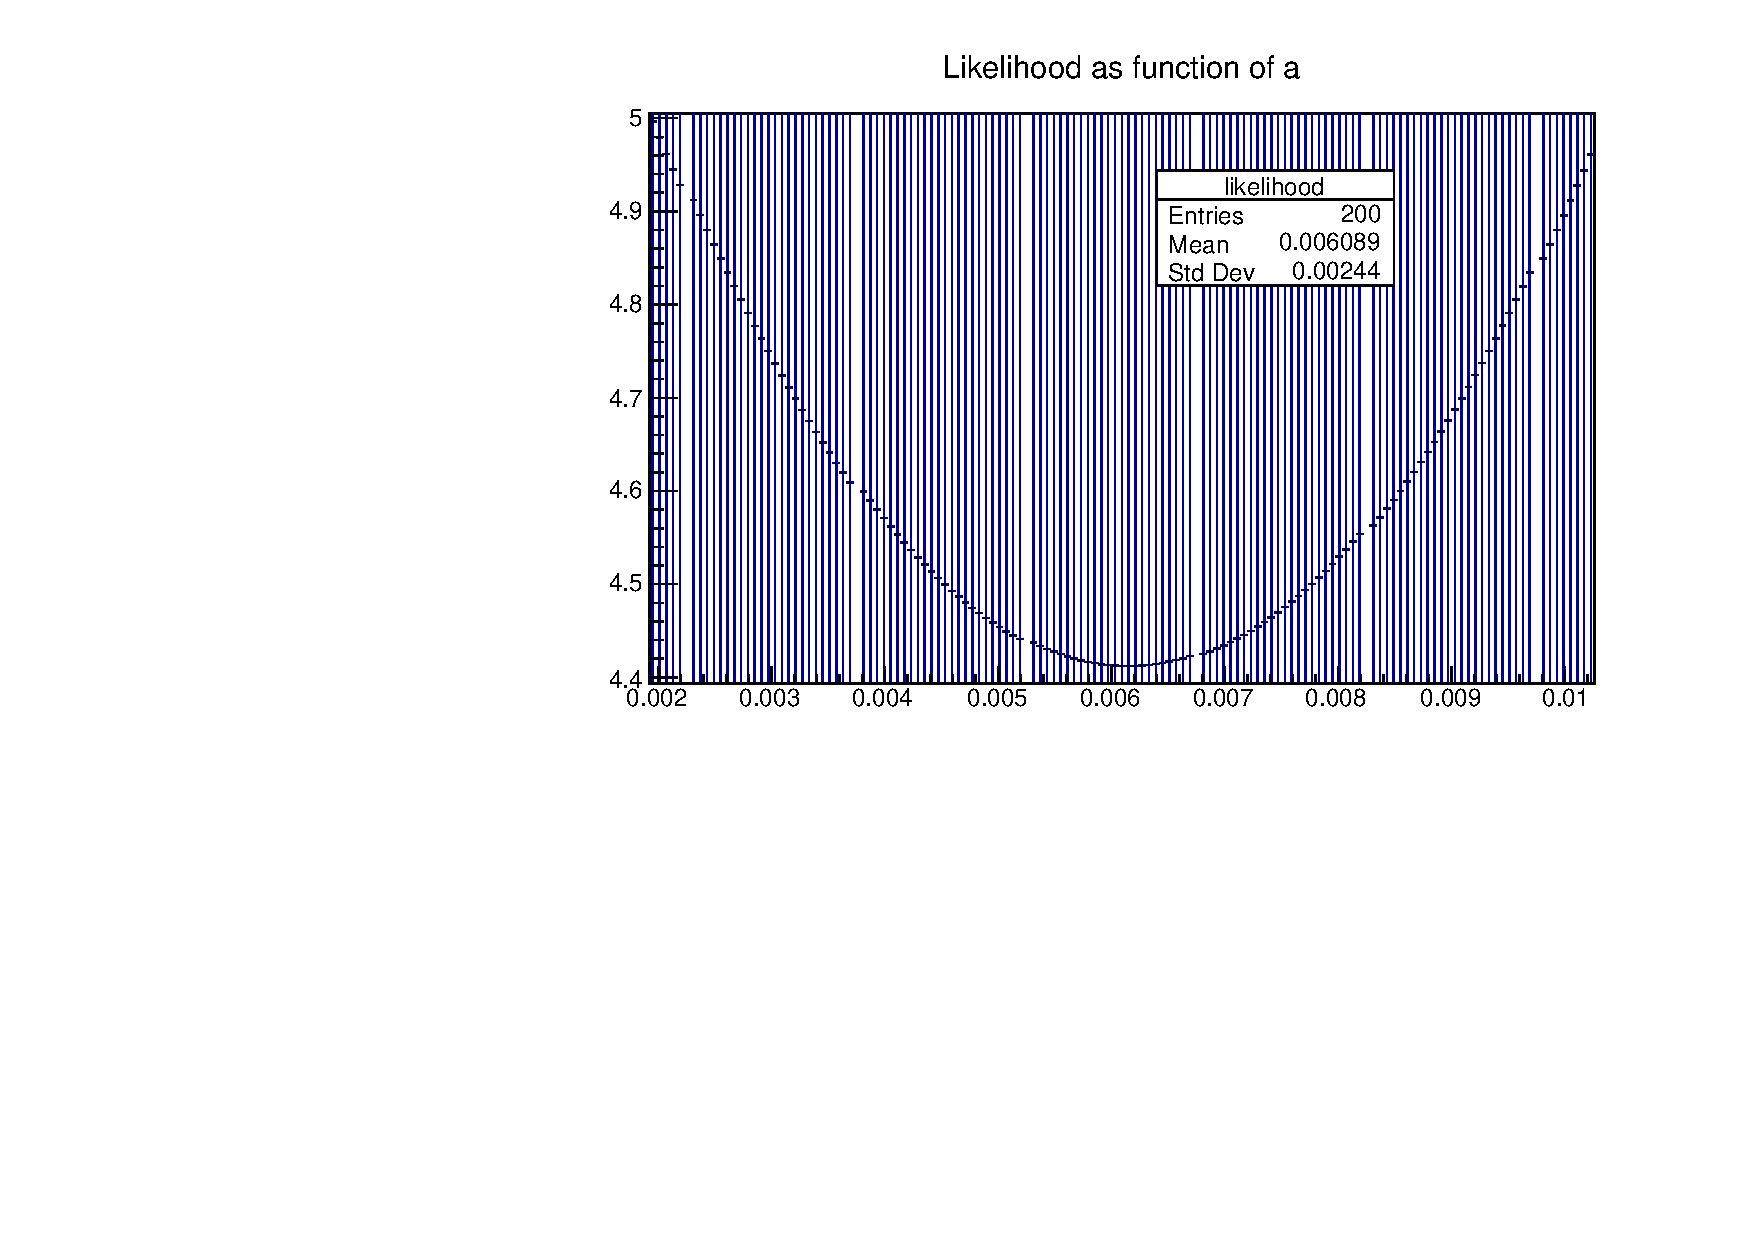
\includegraphics[scale=0.7]{364likelihood.pdf}
\caption{Likelihood as funcion of $a$ for the one-dimentional fit of the electron distribution with $f_A^Z$ BSM correction.}
\label{03_364likelihood}
\end{figure}

\begin{figure} [htp]
\centering
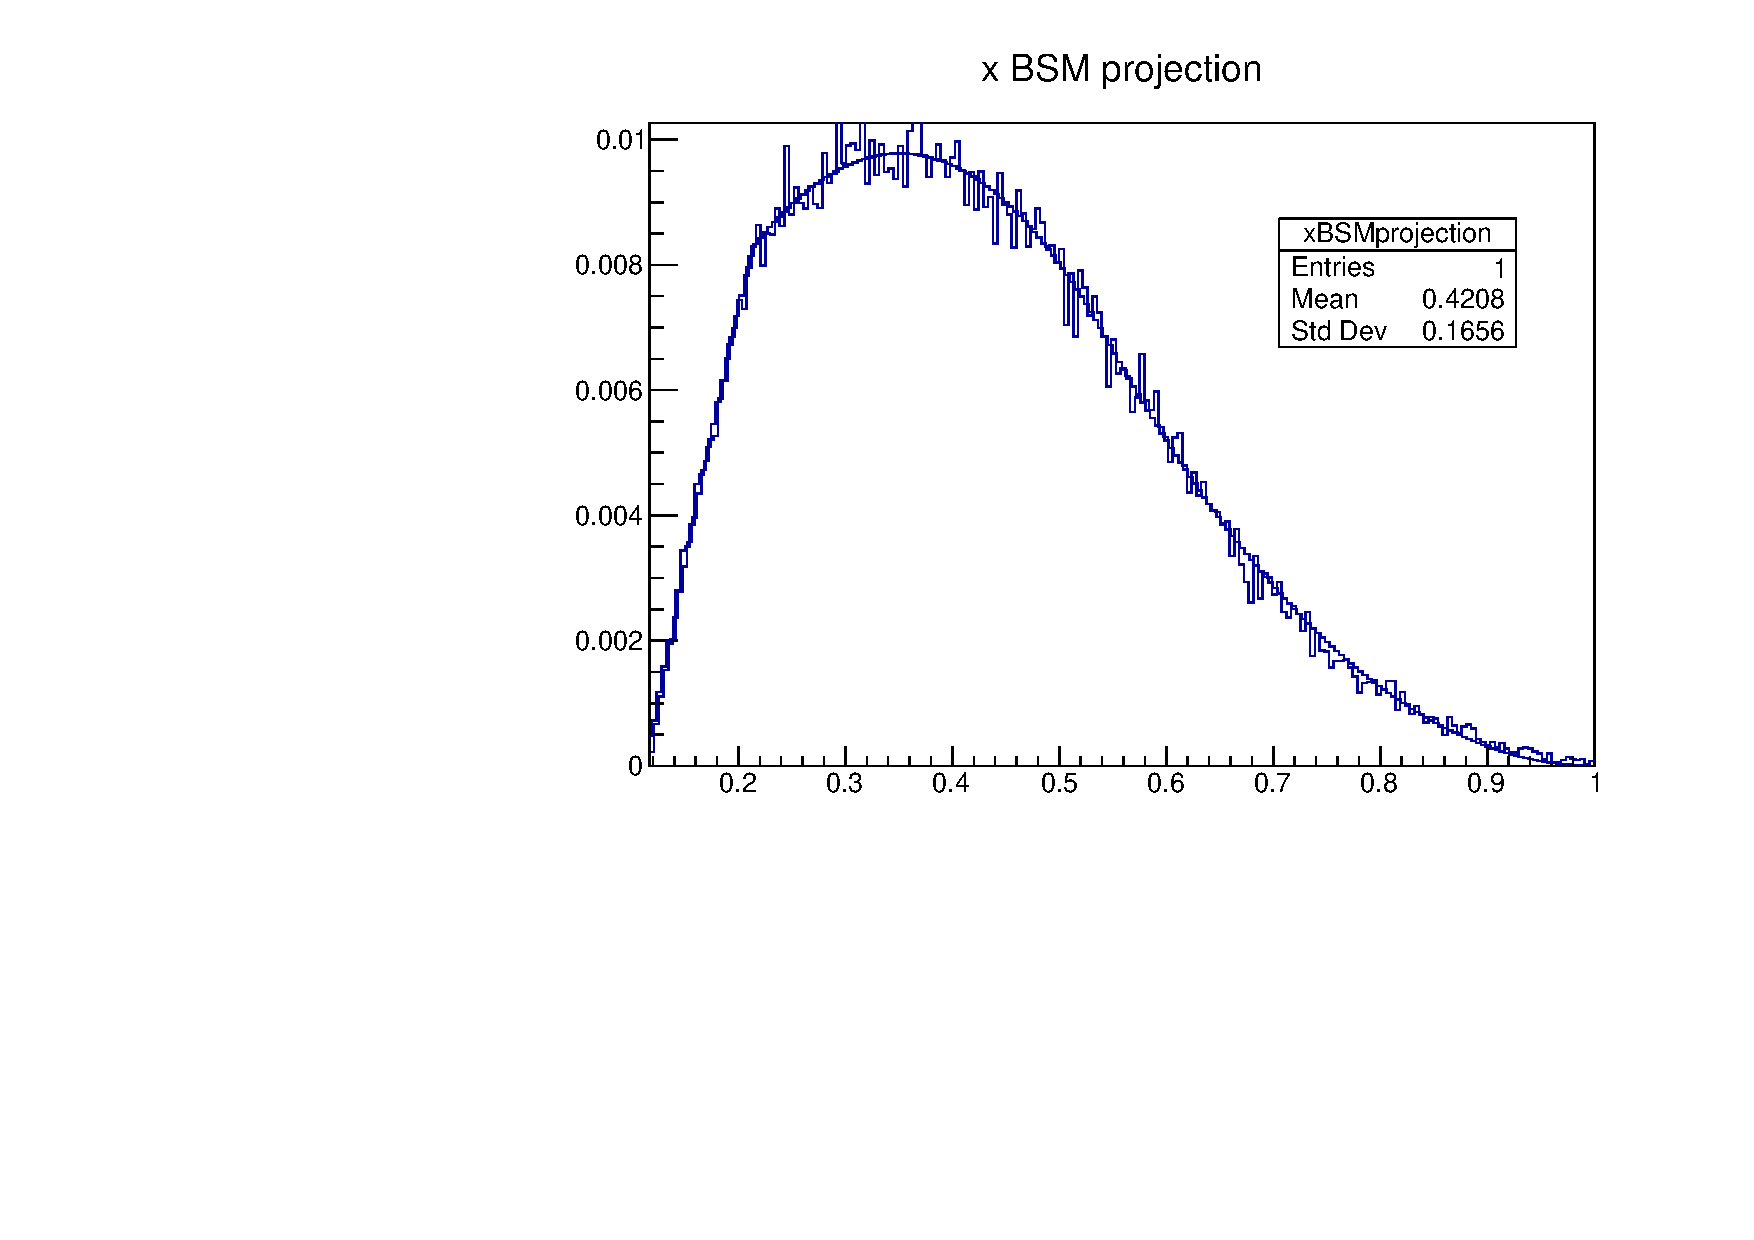
\includegraphics[scale=0.7]{364x.pdf}
\caption{Electrons distribution both simulated and fitted considering the $f_A^Z$ BSM correction, projected on the reduced energy axis.}
\label{03_364x}
\end{figure}

\begin{figure} [htp]
\centering
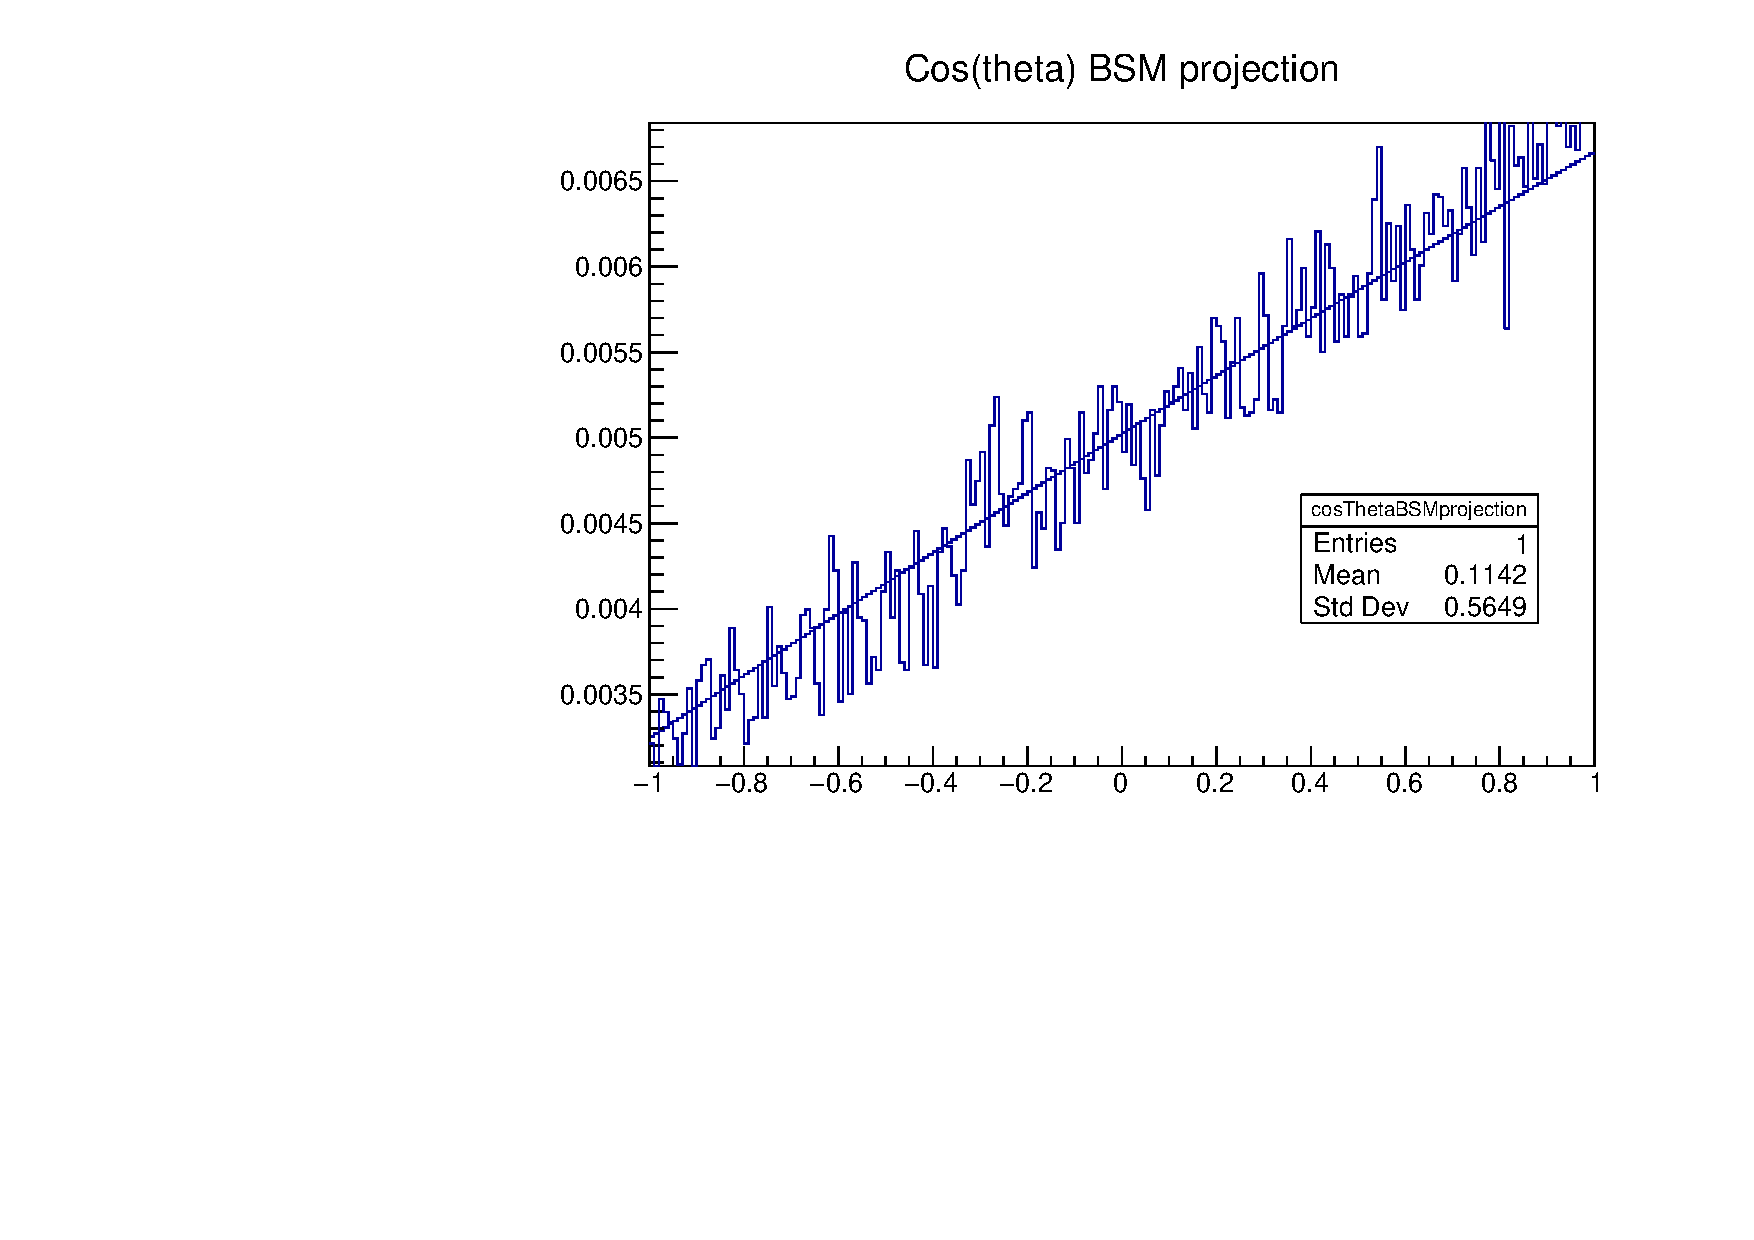
\includegraphics[scale=0.7]{364cosTheta.pdf}
\caption{Electrons distribution both simulated and fitted considering the $f_A^Z$ BSM correction, projected on the $\cos\theta$ axis.}
\label{03_364cosTheta}
\end{figure}

\textbf{Fit 2D}

We have tried to perform the fit with two corrections together. The generalization is simple: \\
in 1D case we have that 
\[ L'(a)=(a-a_0)L''(a_0)\]
that could be rewritten as \[a_0=a- L'(a)/L''(a_0) \simeq a- L'(a)/L''(a) \]
and could be iterated.

in multidimensional case we have that 
\[ \frac{\partial L}{\partial a_i} = \frac{\partial ^2 L}{\partial a_i \partial a_k} (a_k - a0_k)\]
which is a linear system. Then we could solve the system and iterate the process.

The inverse of the $\frac{\partial^2 L}{\partial a_i \partial a_k}$ matrix in the minimum point is the covariance matrix.

We have performed this fit with all the electron/positron data of the montecarlo. The result is:
\[ 
a=\left(
\begin{array}{c}
0.005\\
-0.08\\
\end{array} 
\right)
\]

\[
cova=\left(
\begin{array}{cc}
1.5e-05 & 2.6e-05\\
2.6e-05 & 1.16e-03\\
\end{array}
\right)
\]

\textbf{Plot the 2D ellipse corresponding to a given confidence level}

For a likelihood-fit with 2 or more dimensions, the area of the ellipse with axis equal to one sigma for each dimension does not correspond to the 68 \% confidence level. The right way is to find the value of a parameter k for which the area under $k \cdot \sigma$ is the confidence level given (for instance 68 \%).

For 2D gaussian one can use the formula $k^2=-2 ln(1-Pr)$ where Pr is the given probability.

In addition here is a table with some k-factor for multidimensional gaussian: \href{https://people.richland.edu/james/lecture/m170/tbl-chi.html}{"Click here"}

So, we have to plot the ellipse \[\left(\frac{x}{\sigma_x}\right)^2 + \left(\frac{y}{\sigma_y}\right)^2 = k^2 \]

In Root is really difficult to plot an ellipse on a canvas with the axis. We have to understand how to do (the TEllipse class it's not very useful...). On Monday we will ask to Patrick and Patrizia to know the most simple way to plot our ellipse.

\subsection{09/08/2015}

\textbf{Particle distance in phase space}

Now we need to find the reconstructed particle that corresponds to "our" lepton. We think that the best way is looping on all the reconstructed charged particle finding the particle that minimize this distance in phase space:
\[ \sqrt{(E-E_{mc})^2 + (\vec{p}-\vec{p_{mc}})^2}\]
where $E_{mc}$ and $p_{mc}$ are the energy and momentum of our lepton.

We have just written a script which fills an histogram with the type, the distance and the difference in energy between the reconstructed particle and the montecarlo lepton.
By trying this script with electron only 99 events I found that the reconstructed particle is mostly an electron, sometimes a photon (5 case) and in a couple of case is a negative pion. I think that the photon are that ones radiated by the electrons, and probably they must be added into the electron energy. A pion could be confused as an electron because it could happen that a charged pion interacting in the electromagnetic calorimeter became a neutral pion that decays immediately in two photons.